\documentclass{article}

\def\ParSkip{} 
% Packages
\usepackage{amssymb,amsmath,amsthm,bbm}
\usepackage{verbatim,float,url,dsfont}
\usepackage{graphicx,subfigure,psfrag}
\usepackage{algorithm,algorithmic}
\usepackage{mathtools,enumitem}
\usepackage{multirow}
\usepackage{ragged2e}
\usepackage{xr-hyper}
\usepackage{array}

\usepackage[colorlinks=true,citecolor=blue,urlcolor=blue,linkcolor=blue]{hyperref}
\usepackage[margin=1in]{geometry}
\usepackage[round]{natbib}

\usepackage[utf8]{inputenc} % allow utf-8 input
\usepackage[T1]{fontenc}    % use 8-bit T1 fonts
\usepackage{booktabs}       % professional-quality tables
\usepackage{nicefrac}         % compact symbols for 1/2, etc.
\usepackage{microtype}      % microtypography

\ifdefined\TimesFont 
\usepackage{times} % use times font
\fi

\ifdefined\ParSkip 
\usepackage{parskip} % use par skip
\fi

% Theorems and such
\newtheorem{theorem}{Theorem}
\newtheorem{lemma}{Lemma}
\newtheorem{corollary}{Corollary}
\newtheorem{proposition}{Proposition}
\theoremstyle{definition}
\newtheorem{remark}{Remark}
\newtheorem{definition}{Definition}

% Assumption
\newtheorem*{assumption*}{\assumptionnumber}
\providecommand{\assumptionnumber}{}
\makeatletter
\newenvironment{assumption}[2]{
  \renewcommand{\assumptionnumber}{Assumption #1#2}
  \begin{assumption*}
  \protected@edef\@currentlabel{#1#2}}
{\end{assumption*}}
\makeatother

% Widebar
\makeatletter
\newcommand*\rel@kern[1]{\kern#1\dimexpr\macc@kerna}
\newcommand*\widebar[1]{%
  \begingroup
  \def\mathaccent##1##2{%
    \rel@kern{0.8}%
    \overline{\rel@kern{-0.8}\macc@nucleus\rel@kern{0.2}}%
    \rel@kern{-0.2}%
  }%
  \macc@depth\@ne
  \let\math@bgroup\@empty \let\math@egroup\macc@set@skewchar
  \mathsurround\z@ \frozen@everymath{\mathgroup\macc@group\relax}%
  \macc@set@skewchar\relax
  \let\mathaccentV\macc@nested@a
  \macc@nested@a\relax111{#1}%
  \endgroup
}
\makeatother

% Min and max 
\DeclareMathOperator*{\argmin}{argmin}
\DeclareMathOperator*{\argmax}{argmax}
\DeclareMathOperator*{\minimize}{minimize}
\DeclareMathOperator*{\maximize}{maximize}
\DeclareMathOperator*{\find}{find}
\DeclareMathOperator{\st}{subject\,\,to}

% Other operators
\DeclareMathOperator{\Cov}{Cov}
\DeclareMathOperator{\Var}{Var}
\DeclareMathOperator{\dm}{dim}
\DeclareMathOperator{\col}{col}
\DeclareMathOperator{\row}{row}
\DeclareMathOperator{\nul}{null}
\DeclareMathOperator{\rank}{rank}
\DeclareMathOperator{\nuli}{nullity}
\DeclareMathOperator{\spa}{span}
\DeclareMathOperator{\sign}{sign}
\DeclareMathOperator{\supp}{supp}
\DeclareMathOperator{\diag}{diag}
\DeclareMathOperator{\aff}{aff}
\DeclareMathOperator{\conv}{conv}
\DeclareMathOperator{\dom}{dom}
\DeclareMathOperator{\tr}{tr}
\DeclareMathOperator{\df}{df}

% Other shortcuts 
\def\R{\mathbb{R}}
\def\C{\mathbb{C}}
\def\E{\mathbb{E}}
\def\P{\mathbb{P}}
\def\T{\mathsf{T}}
\def\half{\frac{1}{2}}
\def\df{\mathrm{df}}
\def\hy{\hat{y}}
\def\hf{\hat{f}}
\def\hmu{\hat{\mu}}
\def\halpha{\hat{\alpha}}
\def\hbeta{\hat{\beta}}
\def\htheta{\hat{\theta}}
\def\indep{\perp\!\!\!\perp}
\def\th{^{\textnormal{th}}}

\def\cA{\mathcal{A}}
\def\cB{\mathcal{B}}
\def\cD{\mathcal{D}}
\def\cE{\mathcal{E}}
\def\cF{\mathcal{F}}
\def\cG{\mathcal{G}}
\def\cK{\mathcal{K}}
\def\cH{\mathcal{H}}
\def\cI{\mathcal{I}}
\def\cL{\mathcal{L}}
\def\cM{\mathcal{M}}
\def\cN{\mathcal{N}}
\def\cP{\mathcal{P}}
\def\cS{\mathcal{S}}
\def\cT{\mathcal{T}}
\def\cW{\mathcal{W}}
\def\cX{\mathcal{X}}
\def\cY{\mathcal{Y}}
\def\cZ{\mathcal{Z}}


\title{Lecture 2: Measures of Dependence and Stationarity \\ \smallskip  
\large Introduction to Time Series, Fall 2023 \\ \smallskip
Ryan Tibshirani}
\date{}

\begin{document}
\maketitle
\RaggedRight
\vspace{-50pt}

Related reading: Chapters 1.3--? of Shumway and Stoffer (SS).

\section{Mean and variance}

\begin{itemize}
\item Given a sequence $x_t$, $t = 1,2,3,\dots$, we define its \emph{mean 
    function} (this is viewed as a function of time) by 
  \[
  \mu_{x,t} = \E(x_t)
  \]
  When it is unambiguous from the context which underlying sequence it refers
  to, we drop the first subscript and simply denote this by $\mu_t$

\item Moreover, we define its \emph{variance function} by
  \[
  \sigma^2_{x,t} = \Var(x_t) = \E[(x_t - \mu_t)^2]
  \]
  Again, when the underlying sequence should be clear from the context, we
  simplify notation and denote this by $\sigma^2_t$

\item The mean and variance functions $\mu_t$ and $\sigma^2_t$ are handy 
  objects, because they tell us about salient features of the time series---the
  drift and spread, respectively, that we should expect over time

\item However, in general, they are not enough to characterize the entire
  distribution of the time series. Why? Two reasons: 

  \begin{enumerate}
  \item In general, the mean and variance are not enough to characterize the
    \emph{marginal} distribution of a single variate $x_t$ along the sequence 

  \item Furthermore, they say nothing about the \emph{joint} distribution of
    two variates $x_s$ and $x_t$ at different times, $s \not= t$. (For example,
    do they tend to go up and down together, or do they tend to repel, or ... ?) 
  \end{enumerate}

  The second of these (joint dependence) we will address soon when we talk about
  autocovariance and stationarity. The first (mean and variance specifying the
  distribution) we will revisit later when we talk about Gaussian processes  

\item Before moving on though, let's look at some examples. First, let's
  consider white noise, which recall, refers to a sequence $x_t$, $t =
  1,2,3,\dots$ of uncorrelated random variables, with zero mean, and constant
  variance. Precisely,   
  \begin{gather*}
  \Cov(x_s, x_t) = 0, \quad \text{for all $s \not= t$} \\
  \E(x_t) = 0, \; \Var(x_t) = \sigma^2, \quad \text{for all $t$} 
  \end{gather*}
  So by definition (this one is kind of vacuous), we have mean function $\mu_t =
  0$ and variance function $\sigma^2_t = \sigma^2$, which are constant functions
  (do not vary in time)

\item How about a moving average of white noise, with window length 3? This is 
  \[
  y_t = \frac{1}{3} \Big( x_{t-1} + x_t + x_{t+1} \Big)
  \]
  Its mean function is
  \begin{align*}
  \mu_t &= \E(y_t)  \\
  &= \frac{1}{3} \Big( \E(x_{t-1}) + \E(x_t) + \E(x_{t+1}) \Big) \\ 
  &= \frac{1}{3} ( 0 + 0 + 0 ) \\
  &= 0
  \end{align*}
  Its variance function is
  \begin{align*}
  \sigma^2_t &= \Var(y_t) \\
  &= \frac{1}{9} \Big( \Var(x_{t-1}) + \Var(x_t) + \Var(x_{t+1}) +{} \\
  &\qquad 2 \Cov(x_{t-1}, x_t) + 2 \Cov(x_t, x_{t+1}) + 2 \Cov(x_{t-1}, x_{t+1}) 
    \Big) \\
  &= \frac{1}{9} ( \sigma^2 + \sigma^2 + \sigma^2 + 0 + 0 + 0) \\
  &= \frac{1}{3} \sigma^2
  \end{align*}
  So its variance is smaller than that of original sequence. In short, smoothing
  reduces variance 

\item This last example might have helped you de-rust on some basic facts about
  expectations and variances. Recall, for constants $a_i$ and random variables
  $x_i$: 
  \begin{gather*}
  \E\bigg( \sum_{i=1}^n a_i x_i \bigg) = \sum_{i=1}^n a_i \E(x_i) \\
  \Var\bigg( \sum_{i=1}^n a_i x_i \bigg) = \sum_{i=1}^n a_i^2 \Var(x_i) + 2
  \sum_{i < j} \Cov(x_i, x_j) 
  \end{gather*}
  The last rule can be thought of as a special case of the more general rule,
  for constants $a_i,b_j$, and random variables $x_i,y_j$: 
  \[
  \Cov\bigg( \sum_{i=1}^n a_i x_i , \sum_{j=1}^m b_j y_j  \bigg) 
  = \sum_{i,j} a_i b_j \Cov(x_i, y_j)
  \]
  (To be clear, the sum on the right-hand side above is taken over $i =
  1,\dots,n$ and $j = 1,\dots,m$) 

\item Ok, one last example before moving on: let's consider a random walk with
  drift,
  \[
  x_t = \delta + x_{t-1} + \epsilon_t
  \]
  for a white noise sequence $\epsilon_t$, $t = 1,2,3\dots$.  Recall, we can
  equivalently write this as (assuming we start at $x_0 = 0$):
  \[
  x_t = \delta t + \sum_{i=1}^t \epsilon_i 
  \] 
  From this, we can see that the mean function is 
  \[
  \mu_t = \delta t + \sum_{i=1}^t \E(\epsilon_i) = \delta t
  \]
  and the variance function is 
  \[
  \sigma^2_t = \sum_{i=1}^t \Var(\epsilon_i) + 2 \sum_{i<j} \Cov(\epsilon_i,
  \epsilon_j) = \sigma^2 t
  \]
  So both the mean and the variance grow over time, proportionally to $t$. 
  Figure \ref{fig:rw} plots example paths over multiple repetitions, for you to
  get a sense of this
\end{itemize}

\begin{figure}[p]
\centering
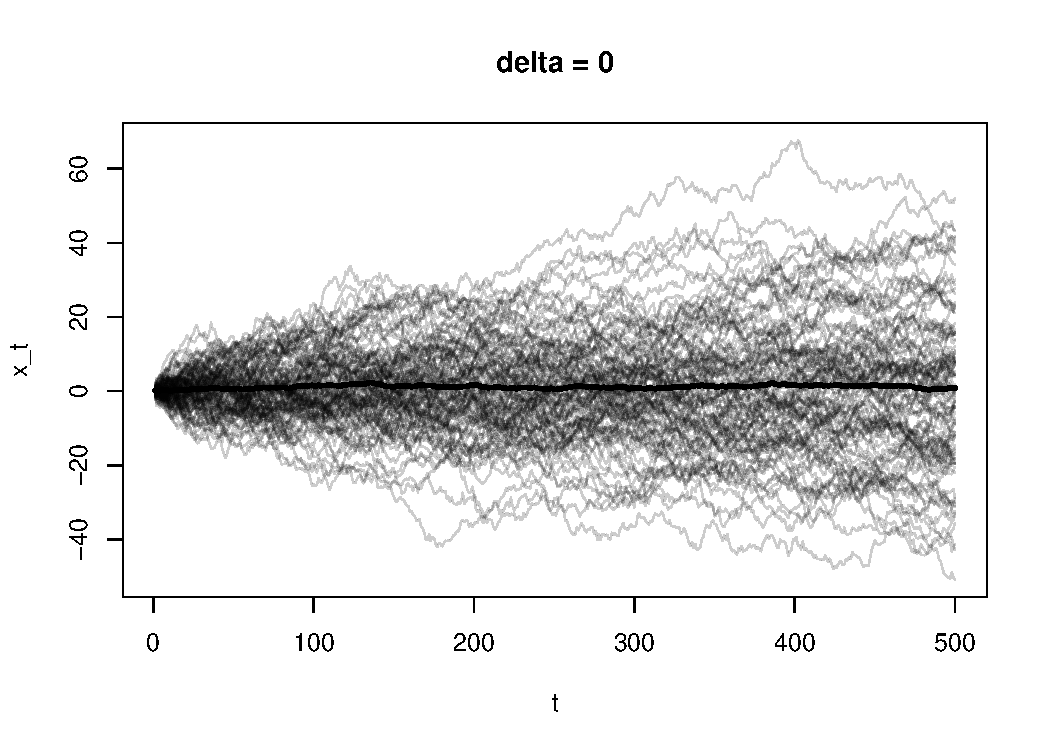
\includegraphics[width=0.85\textwidth]{fig/rw-1.pdf}
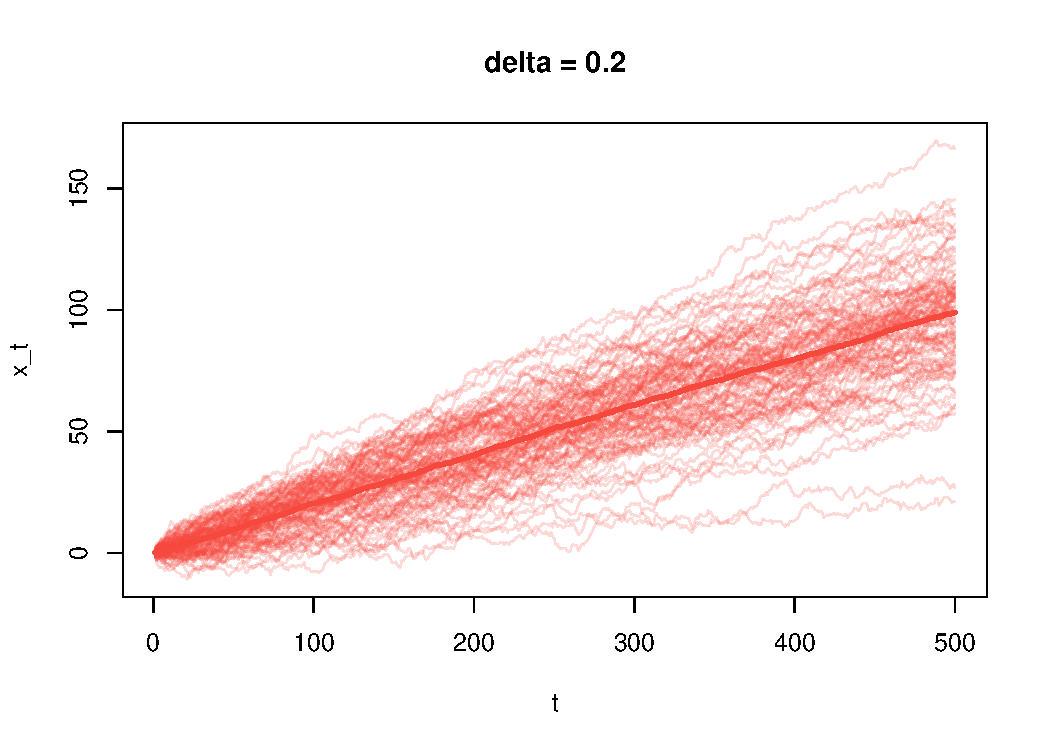
\includegraphics[width=0.85\textwidth]{fig/rw-2.pdf}
\caption{\it Random walk without and with drift, each with 100 sample paths. The
  darker, thicker line in each plot is the sample mean taken at with time point,
  with respect to the 100 repetitions.}
\label{fig:rw}
\end{figure}

\section{Covariance and correlation}

\subsection{Auto: one series}

\subsection{Cross: two series}

\section{Stationarity}

\subsection{Strong}

\subsection{Weak}



\end{document}